%
% The points that I want to cover are the following:
%
% \begin{itemize}
%   \item Building the network from the bioinformatics data and clustering.
%   \item Manipulation of the network: translation and scaling.
%   \item Locomotion and ergonomics used in the VR environment.
%   \item Changing from the blood network to the biopsy network and viceversa.
%   \item Filtering genes in the network using gene sets that represent signatures of cellular pathways which are often dis-regulated in cancer.
% \end{itemize}

%In order to explore the network, several features have been implemented with the purpose of enhance the experience of the visualization process. For example the user has the possibility to move around the network by teleporting to a different place. It is also possible to translate the network and scale it, allowing the user have a better view of the data. The user can also point at a node using the controller to show the name corresponding to that gene or node. Another feature is about entering into a menu where the user can filter the network according to gene sets that represent signatures of cellular pathways which are often dis-regulated in cancer. And finally it is possible also to switch the network from a blood dataset to a biopsy dataset and viceversa.

%The genes nodes in the network and are represented as squared dots and the relationships are represented with lines between them. In Figure \ref{fig:bignet_vr} we can see an example of the application running.

GeneNet VR is a virtual reality application for the interactive visualization of gene networks in a 3D space. The network is represented using nodes and edges between them. In order to explore and visualize the data in GeneNet VR, the user can for example walk around the 3D environment, zoom in the network, translate it to other places, filter the visible nodes using a user interface and also obtain detailed information about the nodes.

GeneNet VR loads the data from local files with the information about the nodes and relationships. Then the network is built using the data and clustered using an algorithm. Finally the user cam explore it and interact with it using the VR headset and controllers.

We implemented GeneNet VR in Unity, a cross-platform game engine. This software is used for a wide range of applications, especially for the development of videogames in 3D and 2D, VR applications and engineering solutions. We used C\# as the main programming language to develop the application in Unity. We also used VRTK, a VR toolkit to build VR solutions in Unity. As for the VR hardware, we used an Oculus Quest headset. This type of headset is an oll-in-one HMD, which means that it doesn't need to be connected to a PC to run an application, it has its own hardware to run the applications although this can be more limited than the hardware from a PC. Also during the development process I used a cable and Oculus Link, a software to connect Oculus Quest to the PC, to run the application and test it directly from Unity on the Oculus Quest, without having to load it to the headset. This was from great help during the development process.

We have chosen two datasets from MIxT to develop GeneNet VR. MIxT is a web application that is used for exploring and comparing bioinformatic data\cite{fjukstad_dumeaux_olsen_lund_hallett_bongo_2017}\cite{dumeaux_fjukstad_interactions_tumor_blood}; and the data visualization is an important part of the process. The datasets used here contain genetic information about a woman with breast cancer. There are in total 2 tissues; the first one is from a blood sample and the second one is from tumor tissue. In Figure \ref{fig:bignet_vr} we can see an example of GeneNet VR running using the blood dataset from MIxT. We will now go in deep with how we implemented GeneNet VR.

\begin{figure}[h!]
    \setlength{\tempheight}{15ex}
    \centering
    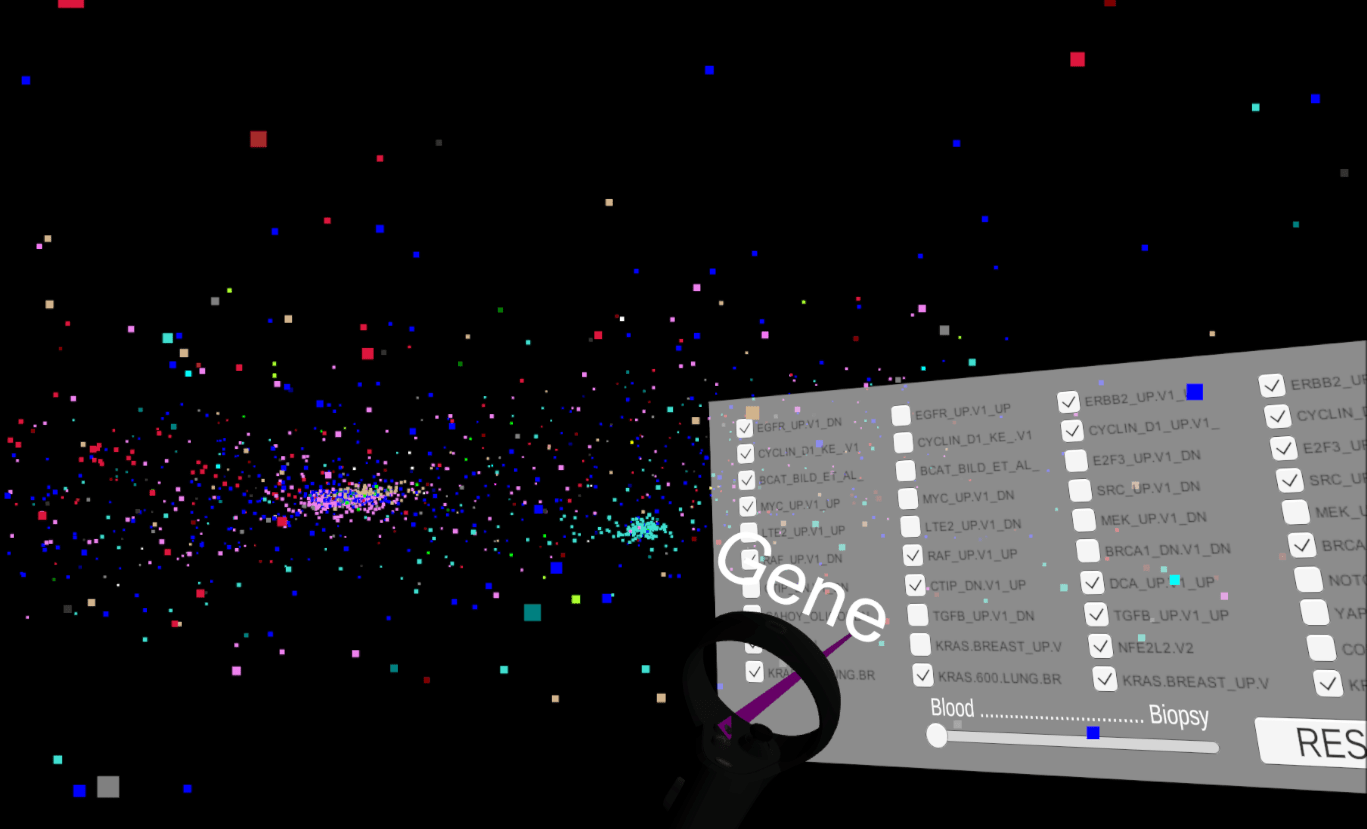
\includegraphics[width=\textwidth]{bignet_vr}
    \caption{GeneNet VR. Example of the application running on a Oculus Quest.}
    \label{fig:bignet_vr}
\end{figure}

\section{Interaction with the network}
Virtual reality headsets offer a rich inmmersive experience. It's not only about inmersing the user into a 3D environment, but also giving the user the possibility to interact with the environment itself. This makes it possible to build complex VR applications where the user can do almost anything in a virtual world. Some examples of what it is possible to do in virtual reality is for example moving around, grabbing objects, interact with the environment using your hands or virtual tools, like pushing a button, 2D interfaces and menus, etc. In this section we will explain the techniques that we have implemented to visualize and interact with the network and make the most of VR.

The interation and the visualization also depends on the VR technoly used. We use Oculus Quest in this project, an all-in-one VR headset that doesn't need a PC nor wires to run the applications. Apart from the headset, it comes with 2 controllers; one for each hand. These controllers have inputs as buttons, thumbsticks and triggers that can be used to activate actions in the VR application. We have used some of these inputs available in the controllers in GeneNet VR and mapped them to different actions that allow the user interact with the network and the environment.

In Figure \ref{fig:oculus_quest_inputs} we can see which actions correspond to each input from the controllers. We will briefly explain now what these actions consist of: 1. Snap rotation: It allows the user to instantly rotate to the right or to the left 45$^{\circ}$; 2. Filter menu: The user can filter the nodes of the network according to a filtering algorithm used in GeneNet VR; 3. Translate network: The network can be translated or moved to other positions in the scene; 4. Scale network: The network can be scaled or "zoomed"; 5. Select node: The user can select a node in order to get more information about it; 6. Select item in menu: It allows the user interact with the menu, for instance to filter the nodes by enabling or disabling the checkboxes from the filtering menu; 7. Oculus menu: It opens the menu from oculus and pauses GeneNet VR; 8. Teleport: It teleports the user to another position on the floor of the VR scene.

As for the use of the Oculus Quest HMD (Head Mounted Display), this is placed in the head and it has a belt that is used to adjust the headset to the head. This will help the user feel more comfortable while wearing the HMD. Another important aspect that we have taken into account in GeneNet VR is that the user can use the application and explore the network by sitting on a chair. This is possible thanks to the locomotion techniques implemented that allows the user to move around with the controllers. We will go into more detail later in this chapter about this.

We will explain now in the following subsections the different interaction techniques that we have used and also what benefits they bring for the visualization and interaction of the network.

\begin{figure}[h!]
    \centering%
    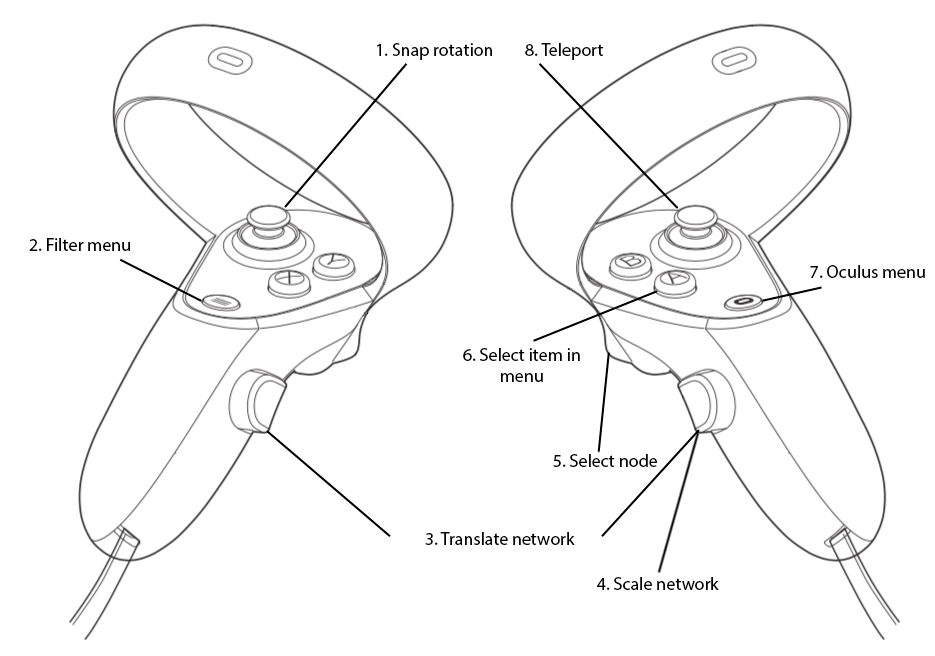
\includegraphics[width=\textwidth]{oculus_quest_inputs}
    \caption{Mapping of the Oculus Quest controllers for the different actions implemented in GeneNet VR: 1. Snap rotation. 2. Filter menu. 3. Scale environment. 4. Translate environment. 5. Pointer. 6. Select item in menu. 7. Oculus menu. 8. Teleport. Adapted figure from Oculus developer's page\cite{oculus_inputs}.}
    \label{fig:oculus_quest_inputs}
\end{figure}%

\subsection{Locomotion}
Locomotion is one of the most important ways of interaction in virtual reality experiences. It can be defined as a self-proppelled movement in the virtual world. Even though moving around is not the main goal in most of VR applications, it is an important aspect for the user's perspective in order to move the user's viewpoint in the virtual world and navigate around it.

Locomotion can have an strong influence in the user's experience. A poorly designed locomotion technique can reduce the user's immersion and even introduce motion sickness, which is related to the movement that the technique produces. HMDs like Oculus Quest allow the users to control the position and the orientation of the viewpoint by moving their heads and walking. However large virtual environments such as GeneNet VR need a big physical tracked area, which cannot be covered by just walking around. It is for this reason that we need to use a locomotion technique that makes it possible to move around without having to walk around in the physical world\cite{locomotion_technique}. in addition, as research has shown, when the user is stationary both in the virtual and real world, the motion sickness produced by VR is less likely\cite{effect_vr_sickness}.

The locomotion technique that we use in GeneNet VR is called teleportation. It consists in choosing a spot on the floor were we want to teleport to. To do this the user has to move forward the thumbstick from the right controller (see "8. Teleport" from Figure \ref{fig:oculus_quest_inputs}). In addition it is possible to choose which direction the user will face once the teleportation is completed. To do this we just need to rotate the same thumbstick to the desired direction. Once the user releases the thumbstick, a black flash will be followed by the new position in the space. This black flash is very important when implementing some of the locomotion techniques because it prevents from producing motion sickness and disorientation. Without the black flash, the transition to the new position would be too abrupt and it may disorient the user.

\begin{figure}[h!]
    \centering%
    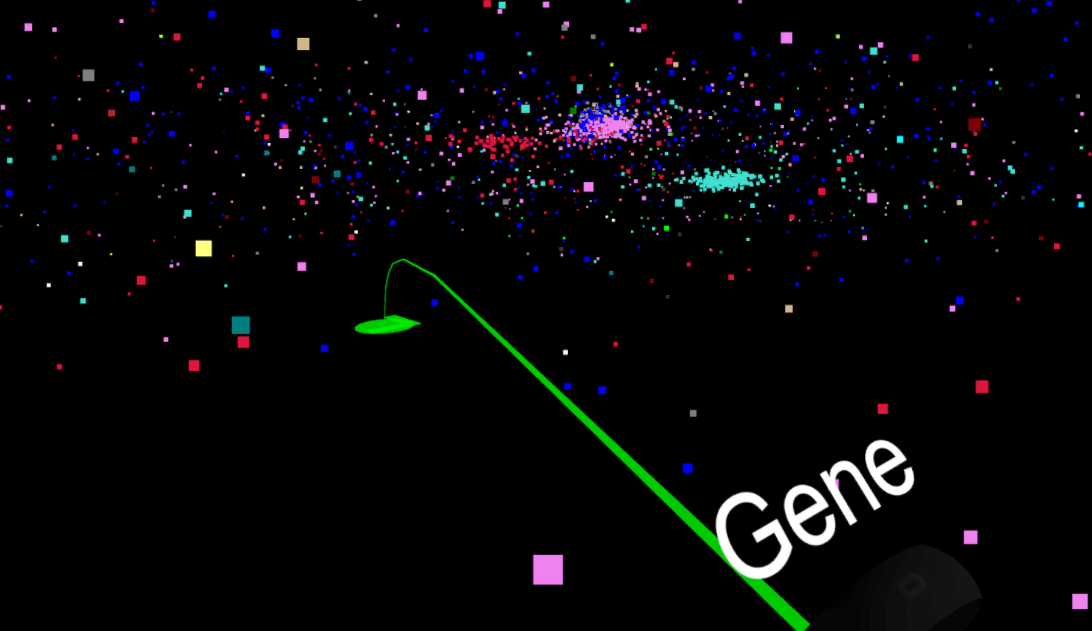
\includegraphics[width=\textwidth]{teleportation2}
    \caption{Teleportation technique. The user can use the jystick from the right controller to teleport to a different spot. To choose the spot a parabolic arc will appear.}
    \label{fig:teleportation}
\end{figure}%

In Figure \ref{fig:teleportation} we can see an example of how the teleportation technique is used in GeneNet VR. A  parabolic arc is created in the 3D space with a circle representing the spot where we are goint to teleport to. It can be seen as if we are throwing an object to the spot where we want to teleport to. The green circle includes also an arrow, indicating the direction that we will face once we are teleported.

In addition to the teleportation, it is also possible to rotate to the left or to the right with the Oculus controllers so that the user doesn't have to rotate the head to look around in the scene. This action is triggered using the thumbstick on the left hand (See 1. Snap rotation in Figure \ref{fig:oculus_quest_inputs}). By moving the thumstick to the left side, the camera will rotate 45$^{\circ}$ to the left side, and 45$^{\circ}$ to the right side if the user moves it to the right side. A black transition is also used in this case before the rotation happens to avoid motion sickness, for the same reason as in the teleportation technique.

\subsection{Translation of the network}
By teleporting to different places in the environment we allow the user visualize the network from different perspectives. However it is also interesting to be able to move the network and specially move it in a precise way so that the user has more control over what it is being visualized. The user might for instance be able to see the network or a specific node or cluster from above or also from below. To do this we have implemented a functionality to translate the network in the 3D space.

\begin{figure}[h!]
    \centering%
    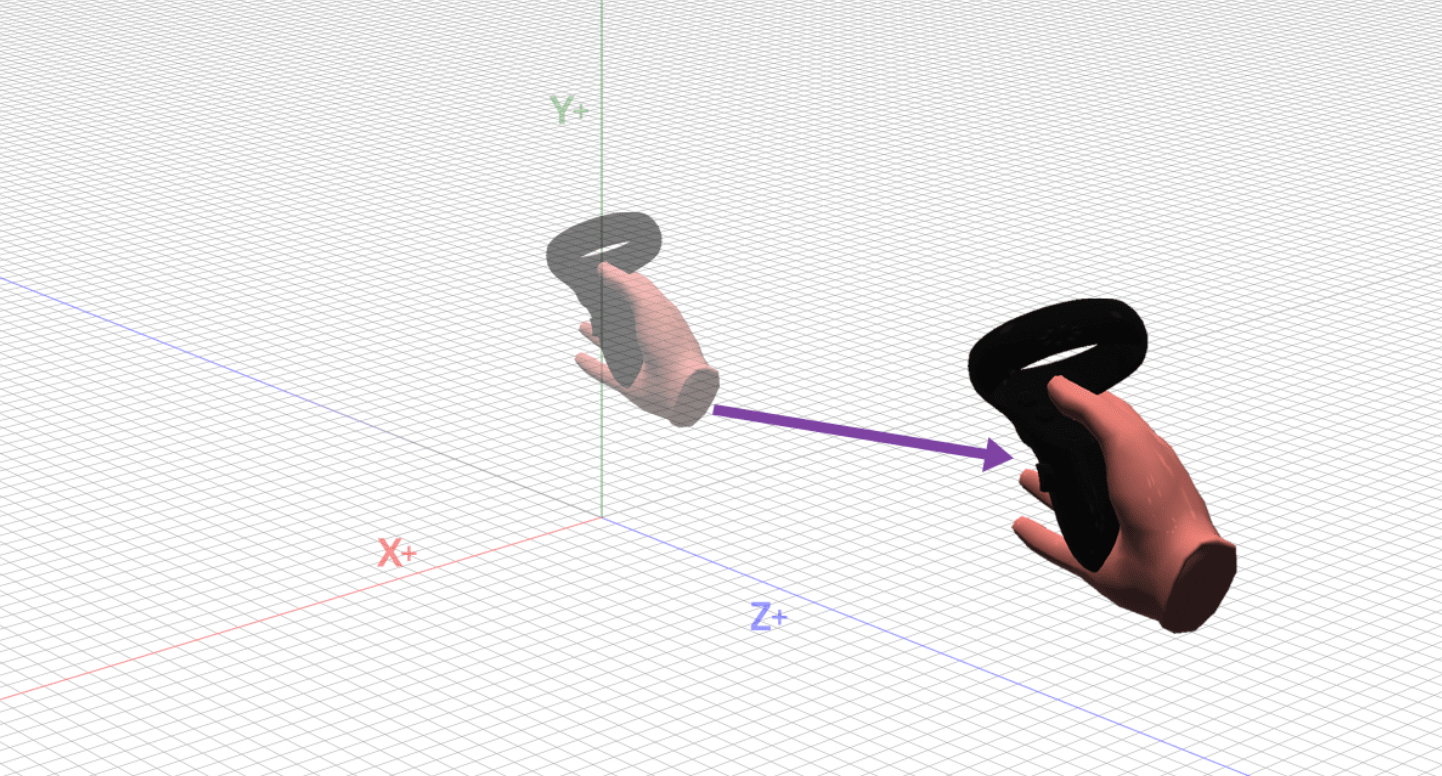
\includegraphics[width=\textwidth]{translation}
    \caption{Translation of the network functionality. The user holds the translation button on the Oculus controller and moves the hand to the direction where he or she wants the network to translate.}
    \label{fig:translation}
\end{figure}%

To translate the network in GeneNet VR, the user needs to press on the hand trigger from the right controller (see "3. Translate network" in Figure \ref{fig:oculus_quest_inputs}). Then the user needs to keep holding this trigger down and move the hand to the direction to which we want the network to move to. This intuitive approach feels like we are just pulling from a rope tied to the network and we just move it to the direction we want.


\subsection{Zooming in the network}
When exploring a big network with hundreds of nodes and several clusters, sometimes the information can be too crowded. In our example dataset that we use in GeneNet VR, there are some clusters of nodes that have too many nodes close to each other and it gets very hard to visualize them properly. A way to cope with this problem is for instance by "zooming" in the part of the network that we want to explore better. We implement then a scaling functionality that makes the network bigger or smaller.

The way we implemented the zooming functionality in GeneNet VR is by using the hand triggers with the name "4. Scale network" (see the reference in Figure \ref{fig:oculus_quest_inputs}). In the first place the user needs to press and hold these triggers from both controllers and then we need to expand or contract the arms, as if we were streching out or contracting the network itself. This is also an intuitive acction to do since the user might think that we are actually stretching the network with the hands.

\begin{figure}[h!]
    \centering%
    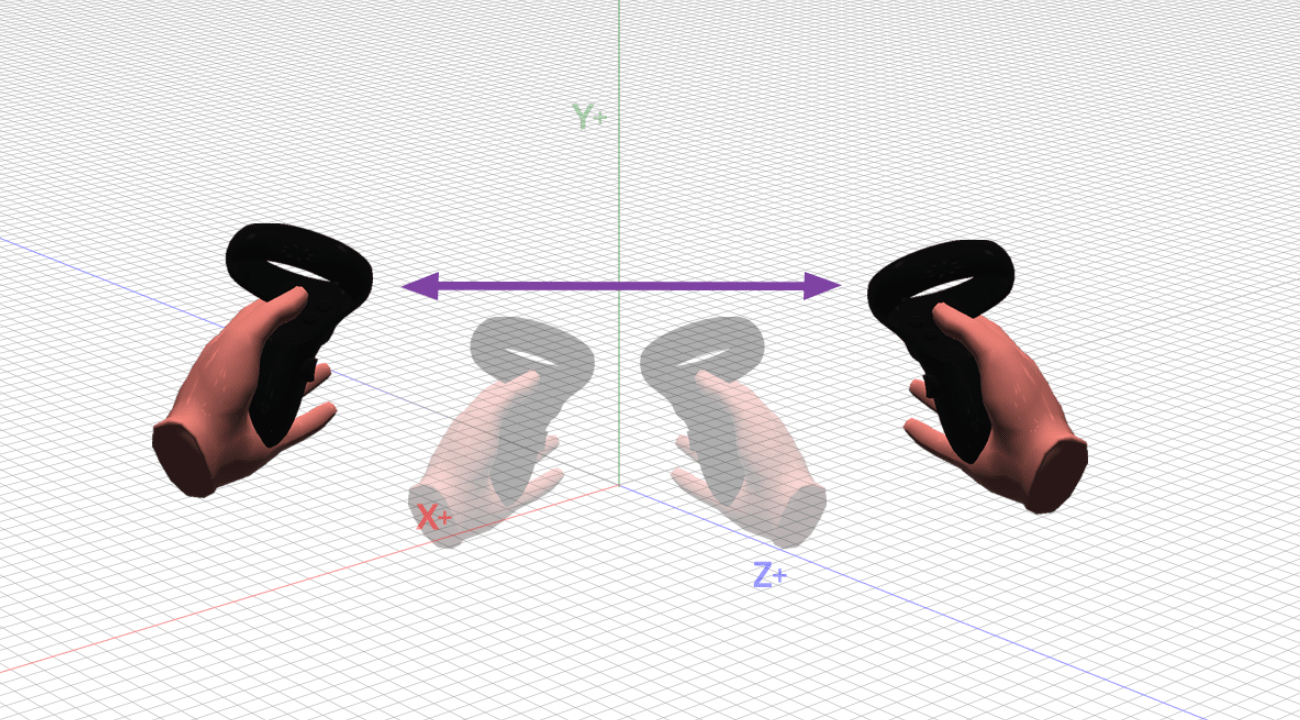
\includegraphics[width=\textwidth]{scaling}
    \caption{Zooming in the network functionality. The user can hold the scaling buttons on the Oculus controller to make the network bigger or smaller. In this example if we strech our hands outside, the network will expand.}
    \label{fig:scaling}
\end{figure}%


In Figure \ref{fig:scaling} there is a visual example of how the zooming works using the Oculus controllers. In this example the user is stretching the hands out in order to make the network bigger. The user starts in a intial position, then holds the zooming triggers from both controllers and then moves the hands out. If we wanted to make the network smaller we would do the opposite action, by contracting the hands to the inside.

\subsection{Interaction with the nodes}
GeneNet VR provides also information about the data that is being displayed. The user can interact with the nodes of the network to obtain information about each of them. In our example, the nodes represent genes and the user might be interested in knowing which gene name corresponds to a specific node. The action that we need to do to obtain the name of the gene is to get close with the right controller to the node that we are interested in and press the "5. Select node" index trigger on the right controller (see Figure \ref{fig:oculus_quest_inputs}). When we press this trigger, we can select a node from the network. By selecting a node, we will get the name of that gene node that will be displayed in a rendered text and we will also visualize the edges from this node to other nodes. The node is selected with an algorithm that searches for the node closest to our right controller.

\subsection{Node relationships}
Finally, our dataset has information about the relationships between the nodes. GeneNet VR is implemented to show also this information. Because there can be too many relationships in the dataset, we don't show them all at the same time. Therefore we can only see those of the node that the user has selected. The way that these relationships are represented is with lines between the nodes.


\section{Scalable network in Unity and data structures}
GeneNet VR uses files from an external source with data that will be used to be the network. The first file contains the information about the nodes and what category the node belongs to; The second one has information about the relationships between each of the nodes. As for the content of the files look like, in Table \ref{tab:categories-data} and Table \ref{tab:network-data} we show an extract from them. Originally the files are in CSV format. CSV\cite{csv} stands for Comma-Separated Values where each record is located on a separate line within the file, delimited by a line break. In addition, each record can contain one or more fields, separated by commas.

For our example we represen the extract from the CSV files using tables, which are more illustrative. Table \ref{tab:categories-data} contains an extract from the file with information about the genes and the categories to which each gene belongs to. Here each row is a category and as we can see, the second cell contains all the gene names for that specific caregory. These categories are named by colors and these color names will be used by GeneNet VR to color each node from the network. As for the second table, Table \ref{tab:network-data}, this one shows an extract with the information about the relationships between the genes. This file can be very large since each row in the CSV file corresponds to a relationship between two genes and one gene can be related with multiple genes. For instance one of the CSV files that GeneNet VR uses to build the relationships contains almost 90k lines.

\begin{table}[h!]
\centering
\begin{tabular}{ll}
\hline
category & genes          \\
brown   & ARHGAP30 FERMT3 ARHGAP25 CD53 PLEK IRF8 DOCK2\\
cyan  & SAFB MOB3A RAB35 ABR ASCC2 CDC37 ANKFY1 GLTSCR1\\
darkgrey  & RAB40C ZNF213 ZNF263 PIGQ RHBDF1 RAB11FIP3\\
darkorange  & TCEB1 MRPL13 ENY2 MTERF3 UBE2W WDYHV1\\
\hline
\end{tabular}
\caption{Fragment of the dataset with the categories and the genes belonging to each category from the biopsy sample.}
\label{tab:categories-data}
\end{table}

\begin{table}[h!]
\centering
\begin{tabular}{llll}
\hline
source & target & weight            & id          \\
AAMP   & ARGLU1 & 0.102486209330144 & AAMP-ARGLU1 \\
ACADM  & FOXN2  & 0.107506881676173 & ACADM-FOXN2 \\
ACADM  & MBNL1  & 0.12269622045714  & ACADM-MBNL1 \\
ACADM  & PPM1B  & 0.103496640767895 & ACADM-PPM1B \\
\hline
\end{tabular}
\caption{Fragment of the dataset used to build the network relationships of the blood sample.}
\label{tab:network-data}
\end{table}

The following diagram shown in Figure \ref{fig:create_network} schematizes the steps that we follow to build the network in Unity. We start with the 2 CSV files described before, containing the data about the nodes and the relationships. We process these CSV files in order to store the data in data structures in GeneNet VR. During the process of storing this data we also apply a clustering algorithm that will set the correct position for each node in the network. After doing this we can easily access the information about the nodes, their position, color and to which nodes they are related to in order to draw the edges. Finally the network is created using a particle system as we will explain later.

\begin{figure}[h!]
    \centering%
    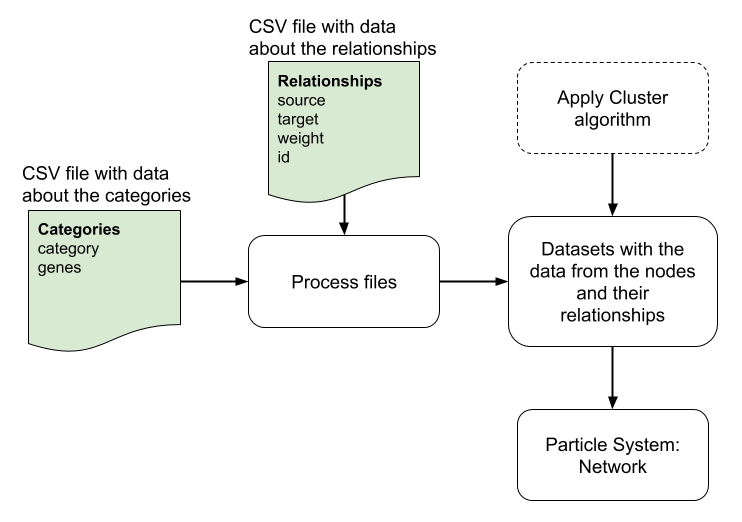
\includegraphics[width=\textwidth]{create_network}
    \caption{Diagram: steps for the creation of the network from the 2 CSV files.}
    \label{fig:create_network}
\end{figure}%

Now that we know how sources of information to build the network in GeneNet VR, let's take a look at how the network itself is represented in Unity and what algorithms and data structures we use for that. These will have an impact in the scalability of the network and therefore it's important to choose a good solution. We have three elements from the network that have more weight in its scalability: the nodes, the edges and the cluster algorithm used. We are going to explain each of them in more detail now.

The nodes in GeneNet VR are represented using a particle system. In Unity a particle system\cite{particle_system} is defined an array of particle ojects. Each particle is a defined structure in Unity that contains properties like the life duration of the particle, start color, start size or position in the 3D space. Particle systems in Unity are very useful to render some special effects like fire, steam, fireworks or projectiles. They are also very powerful because they give plenty of control to the developer over the particles. In GeneNet VR we take advanatge of this, allowing us to structure the network in the way we want. Usually particles have a lifetime, which means that for instance they can start in a position with a particular colour and finish or disappear after a few seconds in a different position and colour. However in GeneNet VR the particles are static and have a very long lifetime, giving the perception that the network is a rigid structure. As for the way the particles are rendered, a 2-dimensional square is shown in the scene for each particle or node. Finally, in order to store the information of each node or particle we have a dictionary object in GeneNet VR that looks like this:

\begin{verbatim}
private Dictionary<string, ParticleSystem.Particle> particles;
\end{verbatim}

A dictionary in C\# is a data structure that contains a set of keys and each key has a single associated value. In our case the key corresponds to the name of the node, the name of the genes in this case, and the value is a particle object.

The edges between the nodes are repsented with 2-dimensional lines in GeneNet VR. A line in Unity is created with a Line Render component\cite{line_render}. These lines are very flexible and can be used to draw anything from a straight line to a spiral. They also have properties like color, texture mode, possibility to have different widths along the line, etc. In our case we want to render straight lines, so we need to know the start and the end points where the line will be rendered. This information is taken from the CSV file with the edges information where we can which nodes are connected to each other. To store the informaion about this we also use a Dictionary, where the key is the name of a node and the value is a list with all the nodes to which this node is connected to. This looks like this in C\#:

\begin{verbatim}
private Dictionary<string, List<string>> edges;
\end{verbatim}

Showing all the edges at the same time in GeneNet VR would make it very hard to visualize the network. For this reason we show only the edges of the node that the user has selected. Also, in GeneNet VR the edges are shown dynamically, meaning that the they are created everytime the user selects a node. When the user selects a different node, the current edges are removed and a new set of edges are rendered for the new node. This process can be a bit CPU-consuming in Unity. Everytime an edge has to be rendered an edge object is instiantated with the CreateInstance method from Unity. The edge object in the scene from what is called a prefab in Unity. A prefab\cite{prefab} is basically a reusable asset, which in our cause is the line with some defines properties like the width and the colour.

The algorithm used to cluster the nodes in the network is another important aspect that can influence in the scalability. In GeneNet VR we use a linear algorithm that clusters the nodes in the 3d space depending on the module where they belong too. In this way the user can visualize each module as single clusters with a distinct colour per cluster.

\section{Other features of GeneNet VR}
GeneNet VR provides some features that help in the process of visualization and interaction with the network. They have a complementary purpose and they don't influence much in the scalability of the system.

\subsection{Filtering information in the network}
Another feature that GeneNet VR uses to improve the visualization of networks is a filtering menu. When we have huge amounts of data in large networks, it is sometimes necessary to show less or more data. By filtering the nodes we can visualize only the part that we are interesting in.

\begin{figure}[h!]
    \centering%
    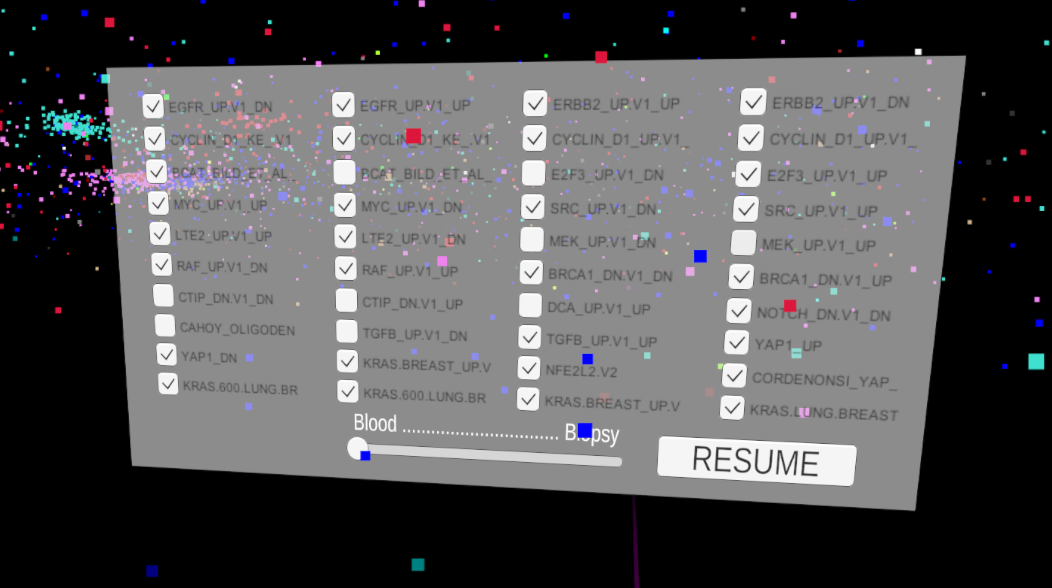
\includegraphics[width=\textwidth]{filtering}
    \caption{Filtering menu in GeneNet VR.}
    \label{fig:filtering}
\end{figure}%

We have built a 2 dimensional menu in Unity, see Figure \ref{fig:filtering}, to filter the data in our example network. We use checkboxes for the filtering. From a starting point, all the boxes are checked, and if the user wants to hide a part from the visualization it is done by unchecking the box. To show the filtering menu we need to press on the menu botton from the left controller, see the "2. Filter menu" in Figure \ref{fig:oculus_quest_inputs}. The to check or uncheck the boxes we need to use the A botton from the right controller, named "6. Select item", see Figure \ref{fig:oculus_quest_inputs}.

\subsection{Network morphing}
Finally GeneNet VR has also the possibility to switch between networks. This can be done in the filtering menu by pressing the menu button from the left controller and there we can see a slider UI element as in Figure \ref{fig:filtering} which we can move to the right or to the left in order to switch the dataset that is being visualized. When we switch the dataset, the filters are also reset to their default state, so all of them will be checked. In our example we can switch from the blood network to the biopsy one.

\section{Implementation details}
Unity (version 2018.4.10f1\cite{unity2018}) is the software that was used to build the system. It is a multi-platform game engine. It is known to be easy to use and for having a big community of creators and asset designers\cite{developing_vr_unity}. Even though it is intuitive to use, it also has a low-level access for developers. As for Virtual Reality, Unity has been up-to-date with the new VR technologies thanks to professionals and amateurs in this area who have built integrations for Unity. In our case, our device is an Oculus Quest, and for this reason we use the Oculus integration for Unity\cite{oculus_unity_integration}. In addition we have used VRTK, a collection of ascripts and assets that help build VR solutions\cite{vrtk_what}. Finally, the programming language used in Unity to implement the system is C\#.

\section{Architecture and design}

\begin{figure}[h!]
    \centering%
    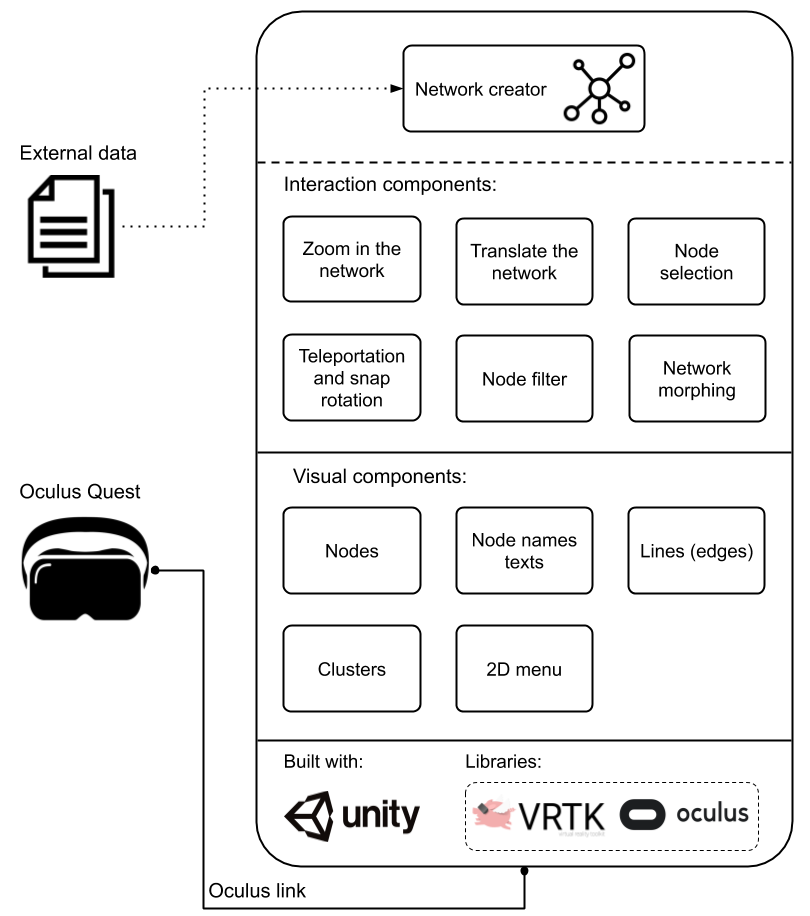
\includegraphics[width=\textwidth]{architecture_design}
    \caption{Architecture and design of GeneNet VR.}
    \label{fig:architecture_design}
\end{figure}%

The architecture for GeneNet VR, as we can see in Figure \ref{fig:architecture_design}, is divided in three parts. The main part is the application built in Unity with VRTK and Oculus libraries. Here is where we have all the logic like the network creator and the interaction features such as zooming, node selector, etc. As for the data used in the application, they come from external files and they have to be manually imported; Then they are processed when starting GeneNet VR, during the network creation. Finally there is the client, which is the Oculus Quest headset where we run GeneNet VR. Here the user can visualize the network and use the controllers to interact with it, using the interaction features that we have created. As the figure shows, the Oculus Quest can be connected to the PC itself using an Oculus Link which is basically a high-quality USB 3 C to C or USB A to C cable with proven performance\cite{oculus_link}. This allows the user run GeneNet VR on the PC. Another possiblity is also load GeneNet VR into the Oculus Quest and run it in the headset hardware without any cable or PC. We are going to explain now in more detail how each of the elements of GeneNet VR were implemented. In this subsection, the actions that are triggered using the Oculus controllers are specified in Figure \ref{fig:oculus_quest_inputs}.

\begin{figure}[h!]
    \centering%
    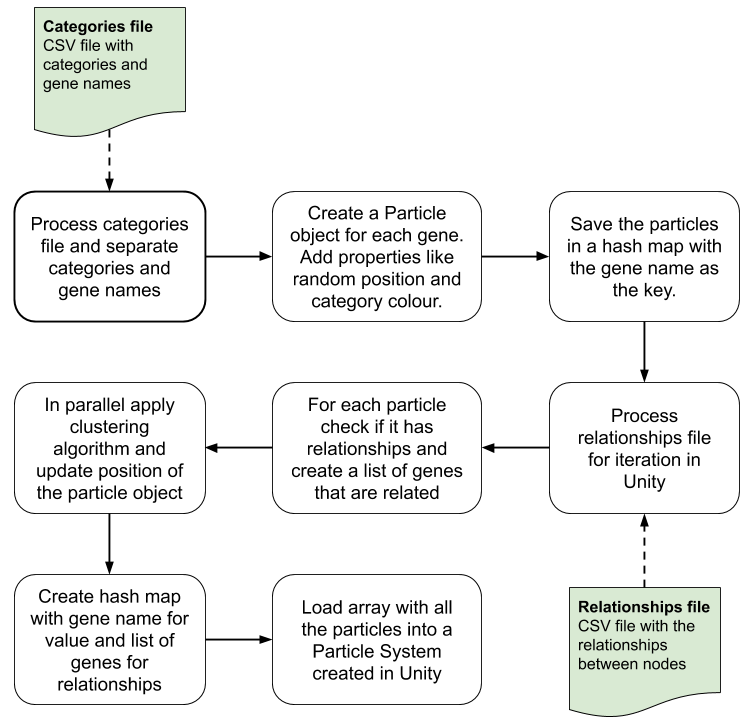
\includegraphics[width=\textwidth]{network_creator}
    \caption{Network creator algorithm.}
    \label{fig:network_creator}
\end{figure}%

The network creator (see Figure \ref{fig:network_creator}) is the component of the application that builds the network from the external data. It processes the data from the CSV files and stores the information in hash maps that can be later be used by the interaction components. During this process of building the network we apply the clustering algorithm as well.

For the \textit{zoom in the network} component I wrote a C\# script where I use the Oculus integration in order to communicate with the controllers of the Oculus Quest. The algorithm is run everytime the user enables the action for zooming (see Figure \ref{fig:network_zoom}). What the script does is to find out if the user is stretching or contracting the arms. For this, when the user triggers the action, the system stores the current position of the left and right controllers in the 3D space and calculates the distance between these 2 points. This position is called initial position. Until the user releases the triggers, the system calculates for every frame the current distance between the two controllers and compares it with the initial distance that was stored right before the user triggered the action. If the new distance one is smaller than the initial one, the network will srink; if it is bigger the network will grow up.

\begin{figure}[h!]
    \centering%
    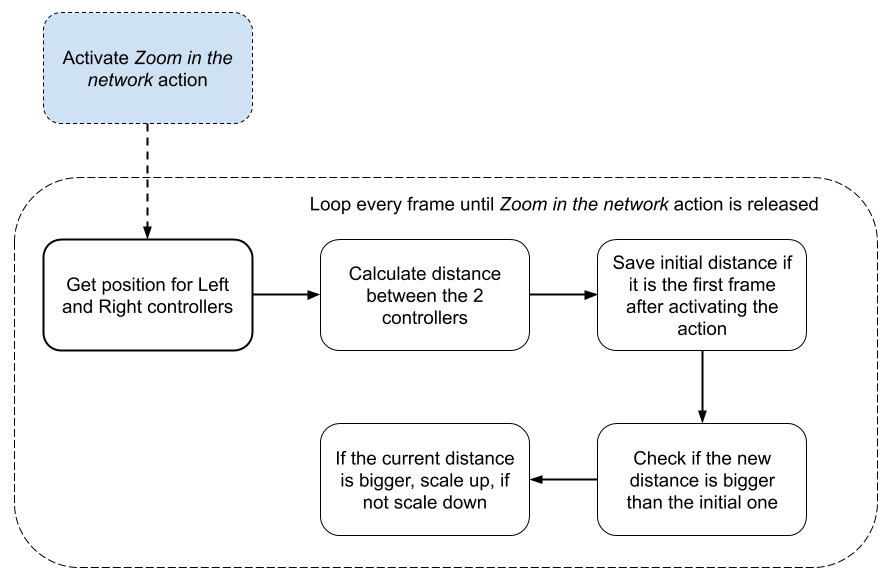
\includegraphics[width=\textwidth]{network_zoom}
    \caption{Algorithm for zooming in the network.}
    \label{fig:network_zoom}
\end{figure}%

For the \textit{translate the network} component I also wrote a script in C\# and using the Oculus integration. Here we do something similar to the \textit{zoom in the network} component. Right before the action is triggered, the position of the right controller is stored as the initial position. Then while the user is holding the trigger of the right controller, the current position for the controller is calculated at every frame. Then a vector is calculated like (current\_position - initial\_position) and normilized. With this we obtained the direction of the vector where the user is trying to move the network to. Then we just add up that vector with a constant to update the position of the network in the 3D space.

\begin{figure}[h!]
    \centering%
    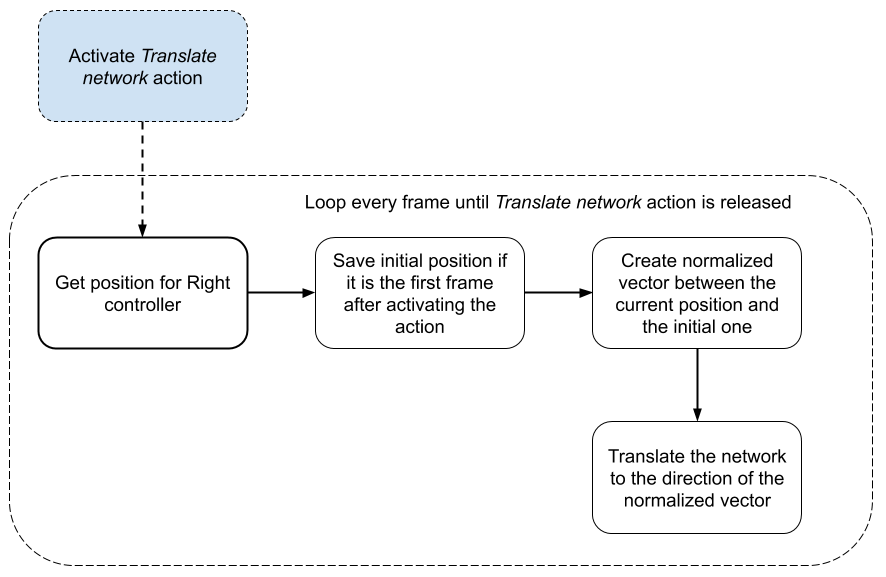
\includegraphics[width=\textwidth]{network_translator}
    \caption{Algorithm for translating the network.}
    \label{fig:network_translator}
\end{figure}%

Select node algorithm:
\begin{figure}[h!]
    \centering%
    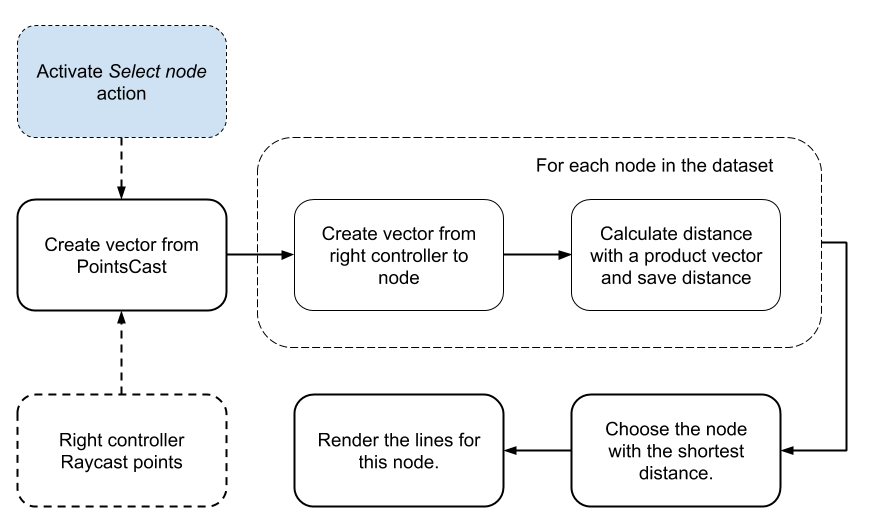
\includegraphics[width=\textwidth]{select_node}
    \caption{Algorithm for the selecton of the nodes in the scene.}
    \label{fig:select_node}
\end{figure}%

For the node filter component, a UI interface is used in Unity. This interface contains several checboxes that are switched on by default. In addition, each checkbox has attached a function that is run everytime the user switches it off or on. This function receives a a text variable as a parameter that is used for the filtering. When the user switches off the checkbox, the algorithm looks into a hash map that looks like this:

\begin{verbatim}
private Dictionary<string, string[]> oncoGroups;
\end{verbatim}

We use the string variable that is passed to the function and that is used to look up the oncoGroups hash map, where each key corresponds to the name of each checkbox. We obtained a list of nodes that we need to turn off from the network.

\section{Discussion}

\subsection{Unity vs Unreal Engine}
Unity3D\footnote{https://unity.com} and Unreal Engine\footnote{https://www.unrealengine.com} are two popular softwares for the development of videogames as well as virtual reality games and other applications. They offer integrations for Oculus Quest and other VR devices in the market.

I chose Unity for the development mostly because I had some experience with it. In addition when I researched about VR development, I found that Unity is good integrated with Oculus Quest and there is the VRTK library. I also found several tutorials about VR development in Unity as well as documentation for the Oculus integration and about VRTK. Unity is also known to be easier to learn. There is a study where they teach Unity and Unreal Engine to students and they conclude that Unity is little less complicated to learn\cite{unity_vs_unreal}. On the other hand Unreal can create more professional looking results. However we are not looking to have realistic graphics in our application since we are dealing with abstract data.

\subsection{VR libraries}
%There are not many libraries available for VR development for Oculus.

\subsection{VR headsets}
We can find numerous VR headsets nowadays in the market\footnote{https://versus.com/en/vr-headset}, from simple headset solutions like Google Cardboard to more advanced ones like HTC Vive Focus. In order to choose which headset we wanted to target our application to, we had into account the price, performance and the features that the headset has. We chose Oculus Quest because the price is not very high (5799,- kr in 2019) and it was also an standalone device, which is not so common among the VR headsets. Oculus Quest also has an advantage as for the performance, it can be connected to a PC where we can run the applications. In this way, this headset is very versatile and the price is affordable for many people and especially for research entities. Other features that Oculus Quest has is that it comes with two controllers that have buttons, triggers and grips that can be used for the interactions in the VR application.
